\section{The VR bound optimisation framework}
This section addresses several issues of the VR bound optimisation by proposing further approximations. First when $\alpha \neq 1$, the VR bound is usually just as intractable as the marginal likelihood for many useful models. However Monte Carlo (MC) approximation is applied here to extend the set of models that can be handled. The resulting method can be applied to any model that MC-VI \cite{paisley:bbvi, salimans:reparam, ranganath:bbvi, kucukelbir:vi_stan} is applied to.
%
Second, Theorem \ref{thm:alpha_vi} suggests that the VR bound is to be minimised when $\alpha < 0$, which performs disastrously in MLE context. As we shall see, this issue is solved also by the MC approximation under certain conditions. Third, a mini-batch training method is developed for large-scale datasets in the posterior approximation context. Hence the proposed optimisation framework of the VR bound enables tractable application to the same class of models as SVI.

\subsection{Monte Carlo approximation of the VR bound}
\label{sec:sampling}
Consider learning a latent variable model with MLE as a running example, where the model is specified by a conditional distribution $p(\bm{x}|\bm{h}, \bm{\varphi})$ and a prior $p(\bm{h}| \bm{\varphi})$ on the latent variables $\bm{h}$. Examples include models treated by the variational auto-encoder (VAE) approach \cite{kingma:vae, rezende:vae} that parametrises the likelihood with a (deep) neural network. MLE requires $\log p(\bm{x})$ which is obtained by marginalising out $\bm{h}$ and is often intractable, so the VR bound is considered as an alternative optimisation objective. However instead of using exact bounds, a simple Monte Carlo (MC) method is deployed, which uses finite samples $\bm{h}_k \sim q(\bm{h}|\bm{x}), k = 1, ..., K$ to approximate $\mathcal{L}_{\alpha} \approx \hat{\mathcal{L}}_{\alpha, K}$:
\begin{equation}
\label{eq:sampling_estimate}
\hat{\mathcal{L}}_{\alpha, K}(q; \bm{x}) = \frac{1}{1 - \alpha} \log \frac{1}{K} \sum_{k=1}^K \left[\left( \frac{p(\bm{h}_k, \bm{x})}{q(\bm{h}_k|\bm{x})} \right)^{1 - \alpha} \right].
\end{equation}
The importance weighted auto-encoder (IWAE) \cite{burda:iwae} is a special case of this framework with $\alpha = 0$ and $K < +\infty$. But unlike traditional VI, here the MC approximation is biased. Fortunately we can characterise the bias by the following theorems proved in the appendix.
%
\begin{theorem}
\label{thm:sampling_bound}
Assume $\mathbb{E}_{\{\bm{h}_k\}_{k=1}^K} [ |\hat{\mathcal{L}}_{\alpha, K}(q; \bm{x})| ] < + \infty$ and $|\mathcal{L}_{\alpha}| < +\infty$. Then $\mathbb{E}_{\{\bm{h}_k\}_{k=1}^K} [ \hat{\mathcal{L}}_{\alpha, K}(q; \bm{x}) ]$ as a function of $\alpha \in \mathbb{R}$ and $K \geq 1$ is: \\
1) \textbf{non-decreasing} in $K$ for fixed $\alpha \leq 1$, and \textbf{non-increasing} in $K$ for fixed $\alpha \geq 1$; \\
2) $\mathbb{E}_{\{\bm{h}_k\}_{k=1}^K} [ \hat{\mathcal{L}}_{\alpha, K}(q; \bm{x}) ] \rightarrow \mathcal{L}_{\alpha}$ as $K \rightarrow +\infty$; \\
3) \textbf{continuous} and \textbf{non-increasing} in $\alpha$ with fixed $K$.
\end{theorem}
%
\begin{corollary}
\label{thm:alpha_k_existence}
For finite $K$, either $\mathbb{E}_{\{\bm{h}_k\}_{k=1}^K} [ \hat{\mathcal{L}}_{\alpha, K}(q; \bm{x}) ] < \log p(\bm{x})$ for all $\alpha$, or there exists $\alpha_K \leq 0$ such that $\mathbb{E}_{\{\bm{h}_k\}_{k=1}^K} [ \hat{\mathcal{L}}_{\alpha_K, K}(q; \bm{x}) ] = \log p(\bm{x})$ and $\mathbb{E}_{\{\bm{h}_k\}_{k=1}^K} [ \hat{\mathcal{L}}_{\alpha, K}(q; \bm{x}) ] > \log p(\bm{x})$ for all $\alpha < \alpha_K$. Also $\alpha_K$ is \textbf{non-decreasing} in $K$ if exists, with $\lim_{K \rightarrow 1} \alpha_K = -\infty$ and $\lim_{K \rightarrow +\infty} \alpha_K = 0$.
\end{corollary}

%
The intuition behind the theorems is visualised in Figure \ref{fig:divergence_sampling}. By definition, the exact VR bound is a lower-bound or upper-bound of $\log p(\bm{x})$ when $\alpha > 0$ or $\alpha < 0$, respectively. However the MC approximation $\mathbb{E}[\hat{\mathcal{L}}_{\alpha, K}]$ biases the estimate towards $\mathcal{L}_{\text{VI}}$, where the approximation quality can be improved using more samples. Thus for finite samples and under mild conditions, negative alpha values can potentially be used to improve the accuracy of the approximation, at the cost of losing the upper-bound guarantee.
%
Figure \ref{fig:divergence_simulation} shows an empirical evaluation by computing the exact and the MC approximation of the R{\'e}nyi divergences. In this example $p$, $q$ are 2-D Gaussian distributions with $\bm{\mu}_p = [0, 0]$, $\bm{\mu}_q = [1, 1]$ and $\bm{\Sigma}_p = \bm{\Sigma}_q = \bm{I}$. The sampling procedure is repeated 200 times to estimate the expectation. Clearly for $K = 1$ it is equivalent to an unbiased estimate of the KL-divergence for all $\alpha$ (even though now the estimation is biased for $\mathrm{D}_{\alpha}$). For $K > 1$ and $\alpha < 1$, the MC method under-estimates the VR bound, and the bias decreases with increasing $K$. For $\alpha > 1$ the inequality is reversed also as predicted.


\begin{figure*}[t]
 \centering
 \subfigure[MC approximated VR bounds.]{
 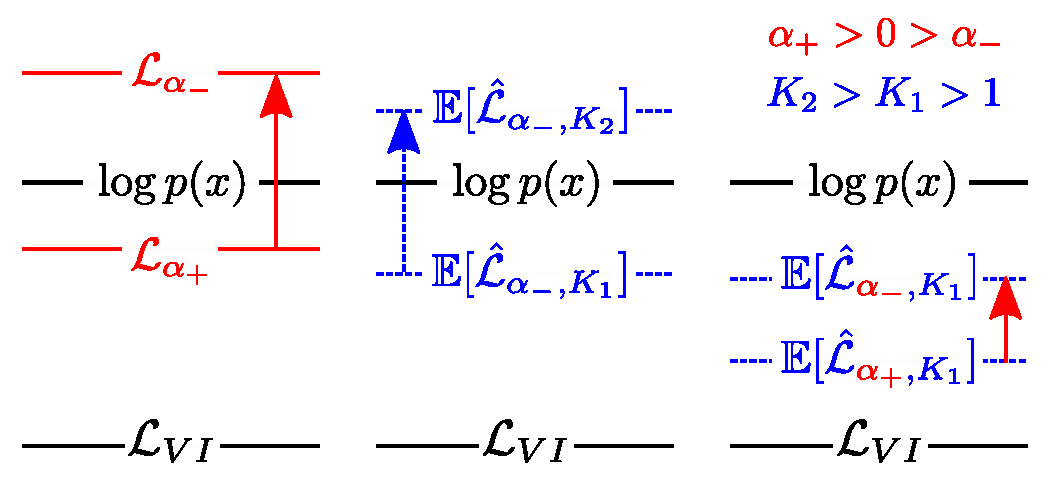
\includegraphics[width=0.6\linewidth]{figs/sampling_bound_full.pdf}
 \label{fig:divergence_sampling}}
 \hspace{0.1in}
 \subfigure[Simulated MC approximations.]{
 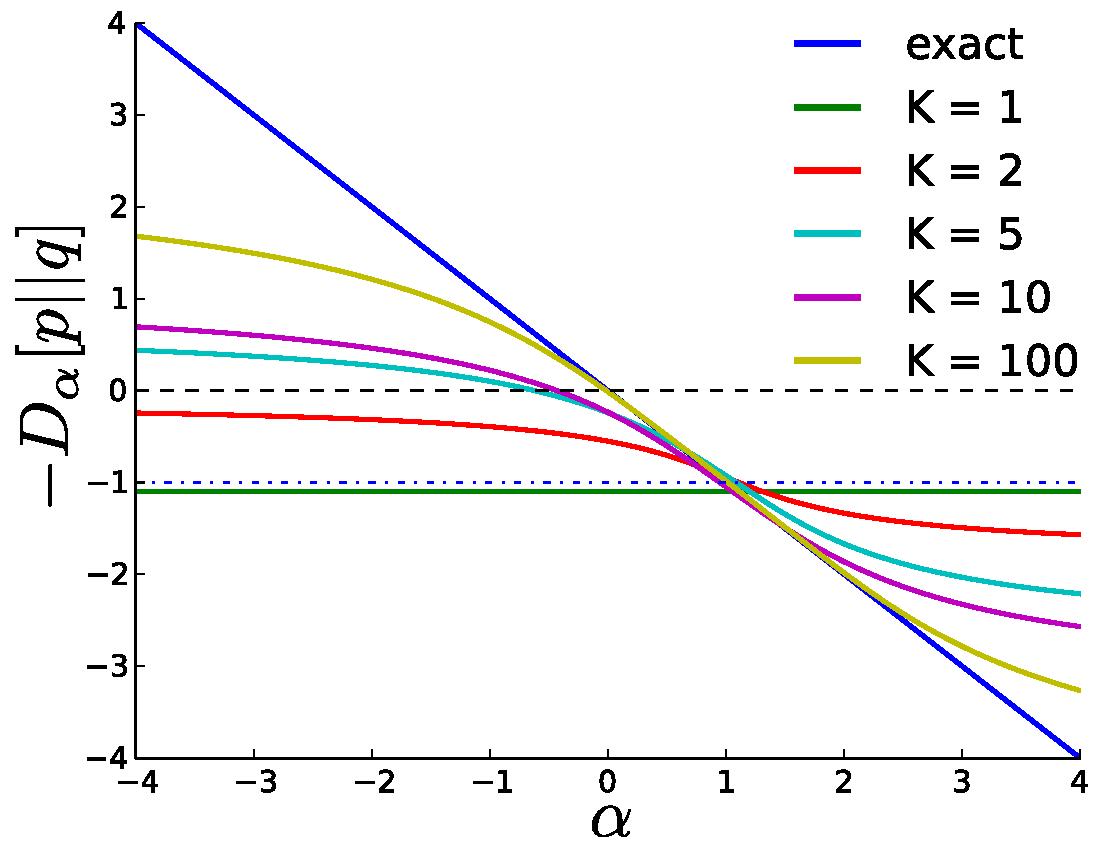
\includegraphics[width=0.34\linewidth]{figs/divergence_sampling.pdf}
 \label{fig:divergence_simulation}}
 \vspace{-0.1in}
 \caption{(a) An illustration for the bounding properties of MC approximations to the VR bounds. (b) The bias of the MC approximation. Best viewed in colour and see the main text for details.}
\end{figure*}

%%%%%%%%%%%%%%%%%%%%
\subsection{Unified implementation with the reparameterization trick}

Readers may have noticed that $\mathcal{L}_{\text{VI}}$ has a different form compared to $\mathcal{L}_{\alpha}$ with $\alpha \neq 1$. In this section we show how to unify the implementation for all finite $\alpha$ settings using the \emph{reparameterization trick} \cite{salimans:reparam, kingma:vae} as an example. This trick assumes the existence of the mapping $\bm{\theta} = g_{\bm{\phi}}(\bm{\epsilon})$, where the distribution of the noise term $\bm{\epsilon}$ satisfies $q(\bm{\theta}) d\bm{\theta} = p(\bm{\epsilon}) d\bm{\epsilon}$. Then the expectation of a function $F(\bm{\theta})$ over distribution $q(\bm{\theta})$ can be computed as
%
$\mathbb{E}_{q(\bm{\theta})} [F(\bm{\theta})] = \mathbb{E}_{p(\bm{\epsilon})} [F(g_{\bm{\phi}}(\bm{\epsilon}))].$
%
One prevalent example is the Gaussian reparameterization: $\bm{\theta} \sim \mathcal{N}(\bm{\mu}, \Sigma) \Rightarrow \bm{\theta} = \bm{\mu} + \Sigma^{ \frac{1}{2} } \bm{\epsilon}, \bm{\epsilon} \sim \mathcal{N}(\bm{0}, I)$. 
%
Now we apply the reparameterization trick to the VR bound
%
\begin{equation}
\mathcal{L}_{\alpha}(q_{\bm{\phi}}; \bm{x}) = \frac{1}{1 - \alpha} \log \mathbb{E}_{\bm{\epsilon}} \left[\left( \frac{p(g_{\bm{\phi}}(\bm{\epsilon}) , \bm{x})}{q(g_{\bm{\phi}}(\bm{\epsilon}))} \right)^{1 - \alpha} \right].
\end{equation}
%
Then the gradient of the VR bound w.r.t.~$\bm{\phi}$ is (similar for $\bm{\varphi}$, see appendix for derivation)
\begin{equation}
\nabla_{\bm{\phi}} \mathcal{L}_{\alpha}(q_{\bm{\phi}}; \bm{x}) 
= \mathbb{E}_{\bm{\epsilon}} \left[ w_{\alpha}(\bm{\epsilon}; \bm{\phi}, \bm{x}) \nabla_{\bm{\phi}} \log \frac{p(g_{\bm{\phi}}(\bm{\epsilon}), \bm{x})}{q(g_{\bm{\phi}}(\bm{\epsilon}))} \right],
\label{eq:gradient_reparam}
\end{equation}
%
where $w_{\alpha}(\bm{\epsilon}; \bm{\phi}, \bm{x}) = \left( \frac{p(g_{\bm{\phi}}(\bm{\epsilon}), \bm{x})}{q(g_{\bm{\phi}}(\bm{\epsilon}))} \right)^{1 - \alpha} \bigg/ \mathbb{E}_{\bm{\epsilon}} \left[ \left( \frac{p(g_{\bm{\phi}}(\bm{\epsilon}), \bm{x})}{q(g_{\bm{\phi}}(\bm{\epsilon}))} \right)^{1 - \alpha} \right]$ denotes the normalised importance weight. 
%
One can show that this recovers the the stochastic gradients of $\mathcal{L}_{\text{VI}}$ by setting $\alpha = 1$ in (\ref{eq:gradient_reparam}) since now $w_{1}(\bm{\epsilon}; \bm{\phi}, \bm{x}) = 1$, which means the resulting algorithm unifies the computation for all finite $\alpha$ settings. For MC approximations, we use $K$ samples to approximately compute the weight $\hat{w}_{\alpha, k}(\bm{\epsilon}_k; \bm{\phi}, \bm{x}) \propto \left( \frac{p(g_{\bm{\phi}}(\bm{\epsilon}_k), \bm{x})}{q(g_{\bm{\phi}}(\bm{\epsilon}_k))} \right)^{1 - \alpha}$, $k = 1, ..., K$, and the stochastic gradient becomes
\begin{equation}
\nabla_{\bm{\phi}} \hat{\mathcal{L}}_{\alpha, K}(q_{\bm{\phi}}; \bm{x}) 
= \sum_{k=1}^K \left[ \hat{w}_{\alpha, k}(\bm{\epsilon}_k; \bm{\phi}, \bm{x}) \nabla_{\bm{\phi}} \log \frac{p(g_{\bm{\phi}}(\bm{\epsilon}_k), \bm{x})}{q(g_{\bm{\phi}}(\bm{\epsilon}_k))} \right].
\end{equation}
When $\alpha = 1$, $\hat{w}_{1, k}(\bm{\epsilon}_k; \bm{\phi}, \bm{x}) = 1/K$, and it recovers the stochastic gradient VI method \cite{kingma:vae}.

To speed-up learning \cite{burda:iwae} suggested back-propagating only one sample $\bm{\epsilon}_j$ with $j \sim p_j = \hat{w}_{\alpha, j}$, which can be easily extended to our framework. Importantly, the use of different $\alpha < 1$ indicates the degree of emphasis placed upon locations where the approximation $q$ under-estimates $p$, and in the extreme case $\alpha \rightarrow -\infty$, the algorithm chooses the sample that has the \emph{maximum} unnormalised importance weight. 
%
We name this approach \emph{VR-max} and summarise it and the general case in Algorithm \ref{alg:vr_max}. 
%
Note that VR-max (and VR-$\alpha$ with $\alpha < 0$ and MC approximations) does \emph{not} minimise $\mathrm{D}_{1-\alpha}[p||q]$. It is true that $\mathcal{L}_{\alpha} \geq \log p(\bm{x})$ for negative $\alpha$ values. However Corollary \ref{thm:alpha_k_existence} suggests that the tightest MC approximation for given $K$ has non-positive $\alpha_K$ value, or might not even exist. Furthermore $\alpha_K$ becomes more negative as the mismatch between $q$ and $p$ increases, e.g.~VAE uses a uni-modal $q$ distribution to approximate the typically multi-modal exact posterior.



\begin{figure}[!t]
% UGLY USE OF \vspace & \hspace follows
\begin{minipage}[b]{0.5\linewidth}
\centering
\begin{algorithm}[H] 
\caption{One gradient step for VR-$\alpha$/VR-max with single backward pass. Here $\hat{w}(\bm{\epsilon}_k; \bm{x})$ short-hands $\hat{w}_{0, k}(\bm{\epsilon}_k; \bm{\phi}, \bm{x})$ in the main text.} \small
\label{alg:vr_max} 
\begin{algorithmic}[1] 
	\STATE given the current datapoint $\bm{x}$, sample \\$\bm{\epsilon}_1, ..., \bm{\epsilon}_K \sim p(\bm{\epsilon})$
	\STATE for $k = 1, ..., K$, compute the unnormalised weight
	$$\log \hat{w}(\bm{\epsilon}_k; \bm{x}) = \log p(g_{\bm{\phi}}(\bm{\epsilon}_k), \bm{x}) - \log q(g_{\bm{\phi}}(\bm{\epsilon}_k)|\bm{x})$$
	\STATE choose the sample $\bm{\epsilon}_{j}$ to back-propagate: \\
	if $|\alpha| < \infty$: $j \sim p_k$ where $p_k \propto \hat{w}(\bm{\epsilon}_k; \bm{x})^{1 - \alpha}$ \\
	if $\alpha = -\infty$: $j = \argmax_{k} \log \hat{w}(\bm{\epsilon}_k; \bm{x})$ 
	\STATE return the gradients $\nabla_{\bm{\phi}} \log \hat{w}(\bm{\epsilon}_{j}; \bm{x})$
\end{algorithmic}
\end{algorithm}
\end{minipage}
%
\hfill
\begin{minipage}[b]{0.4\linewidth}
\centering
 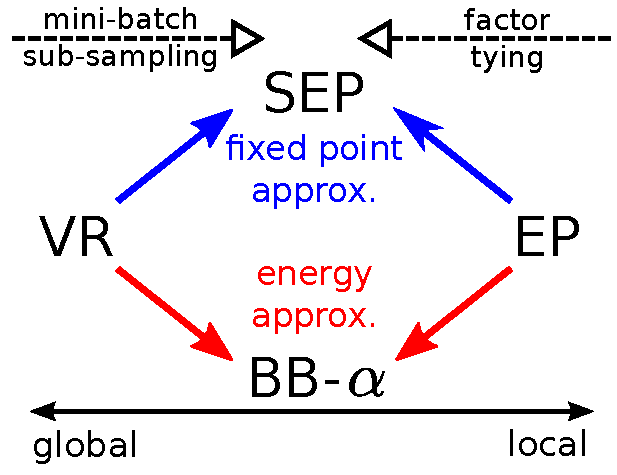
\includegraphics[width=0.9\linewidth]{figs/vr_ep_relationship.pdf} 
 \vspace{-0.1in}
 \captionof{figure}{Connecting local and global divergence minimisation.}
 \label{fig:vr_ep_relationship}
\end{minipage}
%\quad
%
\end{figure}

%%%%%%%%%%%%%%
\subsection{Stochastic approximation for large-scale learning}
\label{sec:large_scale_learning}
VR bounds can also be applied to full Bayesian inference with posterior approximation. However for large datasets full batch learning is very inefficient. Mini-batch training is non-trivial here since the VR bound cannot be represented by the expectation on a datapoint-wise loss, except when $\alpha = 1$. This section introduces two proposals for mini-batch training, and interestingly, this recovers two existing algorithms that were motivated from a different perspective.
%
In the following we define the ``average likelihood'' $\bar{f}_{\mathcal{D}}(\bm{\theta}) = [\prod_{n=1}^N p(\bm{x}_n|\bm{\theta})]^{\frac{1}{N}}$. Hence the joint distribution can be rewritten as $p(\bm{\theta}, \mathcal{D}) = p_0(\bm{\theta}) \bar{f}_{\mathcal{D}}(\bm{\theta})^N$. Also for a mini-batch of $M$ datapoints $\mathcal{S} = \{\bm{x}_{n_1}, ..., \bm{x}_{n_M} \} \sim \mathcal{D}$, we define the ``subset average likelihood'' $\bar{f}_{\mathcal{S}}(\bm{\theta}) = [\prod_{m=1}^M p(\bm{x}_{n_m}|\bm{\theta})]^{\frac{1}{M}}$.

The first proposal considers \emph{fixed point approximations} with mini-batch sub-sampling. It first derives the fixed point conditions for the variational parameters (e.g.~the natural parameters of $q$) using the exact VR bound (\ref{eq:alpha_vi}), then design an iterative algorithm using those fixed point equations, but with $\bar{f}_{\mathcal{D}}(\bm{\theta})$ replaced by $\bar{f}_{\mathcal{S}}(\bm{\theta})$.
%
The second proposal also applies this subset average likelihood approximation idea, but directly to the VR bound (\ref{eq:alpha_vi}) (so this approach is named \emph{energy approximation}):
\begin{equation}
\label{eq:alpha_vi_approx}
\tilde{\mathcal{L}}_{\alpha}(q; \mathcal{S}) 
	= \frac{1}{1 - \alpha} \log \mathbb{E}_{q} \left[ \left( \frac{p_0(\bm{\theta}) \bar{f}_{\mathcal{S}}(\bm{\theta})^N} {q(\bm{\theta})} \right)^{1 - \alpha} \right].
\end{equation}
%
In the appendix we demonstrate with detailed derivations that fixed point approximation returns Stochastic EP (SEP) \cite{li:sep}, and black box alpha (BB-$\alpha$) \cite{hernandez-lobato:bb-alpha} corresponds to energy approximation. Both algorithms were originally proposed to approximate (power) EP \cite{minka:ep, minka:powerep}, which usually minimises $\alpha$-divergences \emph{locally}, and considers $M=1$, $\alpha \in [1 - 1/N, 1)$ and exponential family distributions. These approximations were done by factor tying, which significantly reduces the memory overhead of full EP and makes both SEP and BB-$\alpha$ scalable to large datasets just as SVI. The new derivation derivation provides a theoretical justification from energy perspective, and also sheds lights on the connections between \emph{local} and \emph{global} divergence minimisations as depicted in Figure \ref{fig:vr_ep_relationship}. Note that all these methods recover SVI when $\alpha \rightarrow 1$, in which global and local divergence minimisation are equivalent. Also these results suggest that recent attempts of distributed posterior approximation (by carving up the dataset into pieces with $M > 1$ \cite{gelman:dep, xu:sms}) can be extended to both SEP and BB-$\alpha$.

%
Monte Carlo methods can also be applied to both proposals. For SEP the moment computation can be approximated with MCMC \cite{gelman:dep, xu:sms}. For BB-$\alpha$ one can show in the same way as to prove Theorem \ref{thm:sampling_bound} that simple MC approximation in expectation lower-bounds the BB-$\alpha$ energy when $\alpha \leq 1$. In general it is also an open question how to choose $\alpha$ for given the mini-batch size $M$ and the number of samples $K$, but there is evidence that intermediate $\alpha$ values can be superior \citep{bui:dgp, depeweg:bnn_rl}.